\documentclass[a4paper,12pt,english]{article}
% *** LANGUAGE PACKAGES ***
\usepackage{babel}
\usepackage[utf8]{}
\usepackage[T1]{fontenc}
\usepackage{csquotes}
\usepackage{lmodern}		% Great font
\renewcommand*\familydefault{\sfdefault}
\usepackage[useregional]{datetime2}		% To use several date formats
\usepackage{textcomp, gensymb}
\usepackage{ragged2e}
\usepackage{multicol}
\setlength{\columnsep}{0.5cm}
\setlength{\parindent}{0pt}
\usepackage[dvipsnames,table]{xcolor}


% *** GEOMETRY PACKAGES ***
\usepackage{geometry}
\geometry{left=25mm,
	right=25mm,
	top=35mm,
	bottom=30mm,
	headheight = 35 mm
} 
\usepackage{lastpage}

% *** COLOR PACKAGES ***
\usepackage[most]{tcolorbox}
% Color definitions
\definecolor{blue}{RGB}{0,89,140}
\definecolor{gray}{RGB}{242,242,242}
\definecolor{grayblack}{RGB}{50,50,50}
\definecolor{blue2}{RGB}{10,62,157}
\definecolor{red2}{RGB}{173,17,0}
\definecolor{gray2}{RGB}{230,230,230}
\definecolor{mauve}{rgb}{0.58,0,0.82}
\definecolor{dkgreen}{rgb}{0,0.6,0}

% *** GRAPHICS RELATED PACKAGES ***
\usepackage{graphicx}       % Loading images
\usepackage{float}          % Figures inside minipages
\usepackage{wrapfig}		% Text wrapped around figure
\usepackage{tikz}			% Used to load cover figure
\usepackage{pgfplots}
\pgfplotsset{compat=1.18}

\usepackage[hypcap,font={color=grayblack}]{caption} % used to style the captions
\usepackage{subcaption} 	% For subfigures
\usepackage{overpic}		% To add text over figures
\graphicspath{{images/}}  % Figures relative directory

% *** HEADING AND FOOTER ***
\usepackage{fancyhdr} % For heading and footers
\renewcommand{\headrulewidth}{0.5pt}
\let\oldheadrule\headrule% Copy \headrule into \oldheadrule
\renewcommand{\headrule}{\color{grayblack}\oldheadrule}% Add colour to \headrule
\renewcommand{\footrulewidth}{0.5pt} 
\let\oldfootrule\footrule%
\renewcommand{\footrule}{\color{grayblack}\oldfootrule}% Add colour to \headrule
\pagestyle{fancy}                    % Default page style
\cfoot{}                             % Empty foot center  
\lhead{
\includegraphics[scale=0.1]{QubeCL_Logo.pdf}}     
\rhead{\textcolor{grayblack}{\small \AppNoteNumber}}        
%\lfoot{\textcolor{grayblack}{\DTMsetstyle{ddmmyyyy} \date}}
\lfoot{\textcolor{grayblack}{Revision \vhCurrentVersion}}
\rfoot{\textcolor{grayblack}{\small Pag. \thepage\ - \pageref*{LastPage}}} 			     % Total of pages



% *** TITLE PACKAGES ***
\usepackage{titlesec}
\titleformat{\section}{\color{grayblack}\normalfont\Large\bfseries}{\thesection}{1em}{}
\titleformat{\subsection}{\color{grayblack}\normalfont\large\bfseries}{\thesubsection}{1em}{}
\usepackage{setspace} % Para ajustar la separación entre líneas del documento

% *** TABLE PACKAGES ***
\usepackage{booktabs}
\usepackage{colortbl}
\usepackage{footnote} % To have footnotes inside tables
\usepackage{array}
\usepackage{multirow}
\usepackage{longtable}
\usepackage{arydshln}

\usepackage{xurl} % Lo cargo antes de hyperref, porque ese ya lo carga también.
\urlstyle{sf} % Estilo de los url pasa a Sans Serif.

\usepackage[colorlinks,
citecolor=cyan,
urlcolor=blue,
linkcolor=grayblack,
citebordercolor={0 0 1},
urlbordercolor={0 1 1},
linktocpage,
hyperfootnotes=true
]{hyperref}

%%% EQUATIONS %%%
\usepackage{amsmath}
\usepackage{amssymb}
\usepackage{siunitx}

%%% Version history %%%
\usepackage[]{vhistory}

%%% Code packages %%%
\usepackage{listings}
\lstset{frame=tb,
  aboveskip=3mm,
  belowskip=3mm,
  showstringspaces=false,
  columns=flexible,
  basicstyle={\small\ttfamily},
  numbers=none,
  numberstyle=\tiny\color{gray},
  keywordstyle=\color{blue},
  commentstyle=\color{dkgreen},
  stringstyle=\color{mauve},
  breaklines=true,
  breakatwhitespace=true,
  tabsize=3
}



\begin{document} 
	% Initial settings, new commands and redefinition of existing commands
\newcommand{\AppNoteNumber}{ ppqSense App.Note no. 1}
\renewcommand{\title}{Communication with QubeCL and QubeDL
                        \newline \large \AppNoteNumber}
\renewcommand{\author}{ppqSense Development Team}
\renewcommand{\date}{Revision \vhCurrentVersion\ , \vhCurrentDate}
\newcommand{\justdate}{\vhCurrentDate}

% Definition of ToC title and figures and tables caption
\renewcommand{\contentsname}{Contents}
\renewcommand{\tablename}{\bfseries Table}
\renewcommand{\figurename}{\bfseries Figure}
\renewcommand{\thefootnote}{\textcolor{grayblack}{\arabic{footnote}}}

% Definition of new commands useful for this document
\newcommand{\QubeModel} {Qube }


\color{grayblack}	% Document text color


	
	\begin{titlepage}
	\thispagestyle{empty} % No header nor footer
	\begin{tikzpicture}[remember picture,overlay]
		\node[anchor=west] at (current page.west)
		{
\includegraphics{images/cover.pdf}};
	\end{tikzpicture} % Load the cover
	\hfill 
	%	Title
	\begin{minipage}{12cm}
		\vspace{5cm} 
		\begin{flushright}
			\begin{spacing}{3}
				{\fontsize{40}{50}\selectfont \title}
			\end{spacing}
		\end{flushright}
	\end{minipage}
	\vfill 
	\hfill
	% Subtitle, author and date
	\begin{minipage}{15cm}
		\begin{flushright}	
			\begin{spacing}{2}
				{\Large \bfseries ppqSense s.r.l} \\ [0.5cm]
				{\author} \\ %[0.1cm]
				{\date} \\ [0.5 cm]
				{
\includegraphics[scale=0.1]{QubeCL_Logo.pdf}}
			\end{spacing}
		\end{flushright}
	\end{minipage}
\end{titlepage}

	\newpage

    \paragraph{}ppqSense distributes its QubeCL and QubeDL laser drivers as an almost plug\&play device. To make it possible to use each driver directly out of the box, ppqSense has developed a Control Software for QubeCL and QubeDL, distributed with each one of the drivers with a dedicated pendrive.
    \newline Nevertheless, it may be possible that more complex instrumental setups need to integrate the control of the Qube inside a bigger control software responsible of the management of the whole experiment.

    \paragraph{}In order to allow each user to fully integrate its Qube inside the experiment, this Application Note describes the Serial Connection of the drivers, along with some simple connection examples with different methods.
    
	\tableofcontents
	\listoftables
    \listoffigures      
	\newpage
    
%----   SECTIONS    ----

    \section{Introduction}

\paragraph{} In order to control, manage and monitor the operations of QubeCL and QubeDL laser drivers, ppqSense distributes a dedicated Control Software which provides an intuitive GUI and gives the user access to all the functionalities of the QubeCL/DL drivers, connecting to them by the mean of an USB serial port. Nevertheless, the Control Software is only meant to give the user direct control over the drivers and does not allow to be integrated into a third party control software.

\paragraph{} Complex experimental setups may need to integrate the control of the Qube into their own control software, in order to perform automatized operations without the constant supervision of a user. In this Application Note, we provide the technical specification to control the QubeCL and QubeDL drivers with a third-party Control Software by the means of the same USB serial port used by ppqSense Qube Control Software, along with some specific examples. This will give the user the ability to fully integrate the Qube inside their experimental setup, controlling it with their own control software regardless of the programming method chosen (both LabVIEW and text-based programming languages such as C and Python can be used to achieve control of the Qubes over the Serial Port).


\begin{tcolorbox}[enhanced,attach boxed title to top center={yshift=-3mm,yshifttext=-1mm},
                    colback=black!5!white, colframe=red!75!black, colbacktitle=red!80!black,
                    title=CAUTION, fonttitle=\bfseries, boxed title style={size=small, 
                    colframe=black!50!black} ]

    The Control Software provided by ppqSense includes some safety features that are useful to prevent any usage of the QubeCl and QubeDL drivers that may harm both the driver itself or the laser connected to it.
    \newline While using a third party control software, the user must be particularly cautious in order to avoid any possibly harmful condition for the driver or the laser.
    \newline Before using any third party control software, ppqSense strongly encourages the user to contact the ppqSense technical support to obaint counseling and advices from the techincal staff.
\end{tcolorbox}


\begin{tcolorbox}[enhanced,attach boxed title to top center={yshift=-3mm,yshifttext=-1mm},
                    colback=black!5!white, colframe=red!75!black, colbacktitle=red!80!black,
                    title=CAUTION, fonttitle=\bfseries, boxed title style={size=small, 
                    colframe=black!50!black} ]

    The QubeCL and QubeDL firmware does not prevent the user from sourcing current to the laser without previously activating the temperature controller, this safety measure is usually performed by the Qube Control Software provided by ppqSense.
    \newline While operating with a third party control software, care must be taken in order to never source current to the laser while the temperature controller module (if present) is not active.
\end{tcolorbox}
    \newpage
    
	\section{Direct Communication}  \label{commands_table_chapter}

\paragraph{} The Qubes operates on the basis of a series of commands received by a computer through the USB Serial Port. Each command is codified with a string, to be as friendly for a user as possible, being easily readable.

\paragraph{} The commands share the same structure, each one being composed by a identifier and a value, separated by a colon character.
\newline
    \begin{center}
        \textbf{[identifier]:[value]}
    \end{center}

\paragraph{} The \textit{identifier} allows to differentiate all the available commands, each one acting on a specific functionality of the connected Qube. The \textit{value} is used in association with the \textit{identifier} to define the operation to be carried out by the Qube (for example \textit{activate} or \textit{deactivate} the modulations) or to pass numerical value to be used by the firmware of the device for its operations (for example laser temperature and bias current \textit{setpoints}). The \textit{value} parameter also differentiates the \textbf{write} commands and the \textbf{queries}.

\begin{itemize}
    \item \textbf{Query:} It is possible to send queries to the Qube in order to receive information about its current status, read digital monitors and request informations about the driver. Not all the available \textbf{identifiers} have an associated query.
    \newline In order to send queries to the Qube, the \textbf{value} of the command must be replaced by the \textbf{?} character, for example:
        \begin{center}
            \textbf{iset:?}
        \end{center}
    \item \textbf{Write commands:} Allow to send the Qube numerical values or commands to enable/disable some of its functionalities, for example:
        \begin{center}
            \textbf{iset:150}
        \end{center}
\end{itemize}




%-------------------------------- \QubeModel  Serial Port Specifications --------------------------------%

\subsection{Serial Port Specifications}
\paragraph{} The ppqSense Control Software communicates with the Qubes by the mean of a Serial Connection. The same port can also be used by a third party software to interact with the driver. The baud rate of the Qubes Serial Port is 115200 bps, which has to be set on the third party software in order for it to work with the driver.
\newline The connection of a third-party software is only possible if the Qube Control Software is not running, otherwise the Serial Port resources is kept busy and it is not accessible from the third party software.




%-------------------------------- \QubeModel  Serial Commands --------------------------------%

\subsection{Serial Commands Specifications}
\paragraph{} User can find all the available commands listed in the subsequent tables. Those commands are the ones that are available for the final user to be integrated in a third party control software or to be used in the Qube Control Software to directly communicate with the driver via the dedicated form in the Advanced tab.
\newline In order for the commands to work, they must be sent at the appropriate Baud Rate and each command must be terminated with the \textbf{\textbackslash n} character.
\newline If a suitable \textit{query} is issued, the Qube replies with a string containing the requested informations. All the strings sent as a reply to a \textit{query} are terminated with the \textbf{\textbackslash r\textbackslash n } characters.





%-------------------------------- Available commands for \QubeModel  current generator --------------------------------%
\subsection{List of available commands}

\begin{center}
    \begin{longtable}{| m{0.1\textwidth} | m{0.15\textwidth} | m{0.05\textwidth} | m{0.4\textwidth} | m{0.15\textwidth}| m{0.05\textwidth} |}
    \caption{Available commands for \QubeModel  current generator.\label{\QubeModel _cmd_table_cm}}\\
    \hline
    \textbf{Cmd} & \textbf{Value} & \textbf{R/W} & \textbf{Action} & \textbf{Output \newline Format} & \textbf{Unit} \\
    \hline \hline
    \multicolumn{6}{|c|}{\textbf{Output Current and Modulations}} \\
    \hline
    id: & ? & R & Returns the identificative code of the instrument & \QubeModel -\#\#\#\# & N.A.\\
    \hline
    ilas: & ? & R & Returns the Output Current value readed from the \QubeModel  monitor. & \#\#\#\#.\#\# & mA \\
    \hline
    \multirow{2}{0.1\textwidth}{iset:}  & ? & R & Returns the Current setpoint. & \#\#\#\#.\#\# & mA \\
                                        \cline{2-6}
                                        & \#\#\#\#.\#\# & W & Sets the Current setpoint. & N.A. & mA \\
    \hline
    \multirow{2}{0.1\textwidth}{iout:}  & on & W & Switches the Current ON. & N.A. & N.A. \\
                                        \cline{2-6}
                                        & off & W & Switches the Current OFF. If the modulations were active, they're also switched OFF. & N.A. & N.A. \\
    \hline
    \multirow{2}{0.1\textwidth}{imax:}  & ? & R & Returns the Output Current Maximum Limit set by the user. & \#\#\#\#.\#\# & mA \\
                                        \cline{2-6}
                                        & \#\#\#\#.\#\# & W & Sets the Output Current Maximum Limit. & \#\#\#\#.\#\# & mA \\
    \hline
    vlas: & ? & R & Returns the measured Voltage Drop across the laser & \#\#\#\#.\#\# & V \\
    \hline
    \multirow{2}{0.1\textwidth}{mod:}   & on & W & Enables the overall Modulation Switch. This command becomes active 10 seconds after.                                              the use of the \textbf{iout:on} command. &  N.A. & N.A. \\
                                        \cline{2-6}
                                        & off & W & Disables the overall Modulation Switch. If some of the modulations are active, they are switched off too. & N.A. & N.A. \\
    \hline 
    \multirow{2}{0.1\textwidth}{mod1:}   & on & W & Enables the Modulation Channel 1. &  N.A. & N.A. \\
                                        \cline{2-6}
                                        & off & W & Disables the Modulation Channel 1. & N.A. & N.A. \\
    \hline 
    \multirow{2}{0.1\textwidth}{mod2:}   & on & W & Enables the Modulation Channel 2. &  N.A. & N.A. \\
                                        \cline{2-6}
                                        & off & W & Disables the Modulation Channel 2. & N.A. & N.A. \\
    \hline 
    \end{longtable}
\end{center}





%-------------------------------- Available commands for \QubeModel  temperature controller --------------------------------%

\begin{center}
    \begin{longtable}{| m{0.1\textwidth} | m{0.15\textwidth} | m{0.05\textwidth} | m{0.4\textwidth} | m{0.15\textwidth}| m{0.05\textwidth} |}
    \caption{Available commands for \QubeModel  temperature controller.\label{\QubeModel _cmd_table_tc}}\\
    \hline
    \textbf{Cmd} & \textbf{Value} & \textbf{R/W} & \textbf{Action} & \textbf{Output \newline Format} & \textbf{Unit} \\
    \hline \hline
    \multicolumn{6}{|c|}{\textbf{Laser Temperature Controller}} \\
    \hline
    
    tlas & ? & R & Return the Temperature of the laser measured by the TC Module. & \#\#\#\#.\#\# & \textdegree C \\
    \hline
    
    \multirow{2}{0.1\textwidth}{tstab:} & on & W & Switches the Temperature Stabilization on. & N.A. & N.A. \\
                                        \cline{2-6}
                                        & off & W & Switches the Temperature Stabilization off. & N.A. & N.A. \\
    \hline
    
    \multirow{2}{0.1\textwidth}{tset:} & ? & R & Return the laser Temperature Setpoint & \#\#\#\#.\#\# & \textdegree C \\
                                        \cline{2-6}
                                        & \#\#\#\#.\#\# & W & Sets the laser Temperature Setpoint & N.A. & \textdegree C \\
    \hline
    
    kp: & \#\#\#\#.\#\# & W & Sets the Proportional Gain Coefficient for the digital PID that manages the laser Temperature Stabilization. & N.A. & A/K \\
    \hline
    
    ki: & \#\#\#\#.\#\# & W & Sets the Integral Gain Coefficient for the digital PID that manages the laser Temperature Stabilization. & N.A. & A/Ks \\
    \hline
    
    kd: & \#\#\#\#.\#\# & W & Sets the Derivative Gain Coefficient for the digital PID that manages the laser Temperature Stabilization. & N.A. & As/K \\
    \hline
    
    \multirow{4}{0.1\textwidth}{pid:}   & \multirow{4}{0.15\textwidth}{?} & \multirow{4}{0.05\textwidth}{R} & Returns the Gain Values of the Digital PID that manages the laser Temperature Stabilization. & & \\
                                        & & & kp & \#\#\#\#.\#\#:  & A/K \\
                                        & & & ki & \#\#\#\#.\#\#:  & A/Ks \\
                                        & & & kd & \#\#\#\#.\#\#  & As/K \\
    \hline
    
    \multirow{2}{0.1\textwidth}{tecsign:}   & dir & W & Sets the Temperature Stabilization PID to                                               work in direct mode. & N.A. & N.A. \\
                                        \cline{2-6}
                                            & rev & W & Sets the Temperature Stabilization PID          to work in reverse mode. & N.A. & N.A. \\
    \hline
    
    \multirow{2}{0.1\textwidth}{tlimax:}    & ? & R & Returns the Maximum Temperature Setpoint for the Stabilization PID. & \#\#\#\#.\#\# & \textdegree C \\
                                            \cline{2-6}
                                            & \#\#\#\#.\#\# & W & Sets the Maximum Temperature Setpoint for the Stabilization PID. & N.A. & \textdegree C \\
    \hline
    
    \multirow{2}{0.1\textwidth}{tlimin:}    & ? & R & Returns the Minimum Temperature Setpoint for the Stabilization PID. & \#\#\#\#.\#\# & \textdegree C \\
                                            \cline{2-6}
                                            & \#\#\#\#.\#\# & W & Sets the Minimum Temperature Setpoint for the Stabilization PID. & N.A. & \textdegree C \\
    \hline
    
    \newpage
    
    \hline
    
    \multirow{2}{0.1\textwidth}{teclim:}    & ? & R & Returns the Maximum Current Output for the TC Module. & \#\#\#\#.\#\# & A \\
                                            \cline{2-6}
                                            & \#\#\#\#.\#\# & W & Sets the Maximum Current Output for the TC Module. & N.A. & A \\
    \hline
    
    \multirow{2}{0.1\textwidth}{teslim:}    & ? & R & Returns the threshold for the Active Temperature Error Control. & \#\#\#\#.\#\# & \textdegree C*s \\
                                            \cline{2-6}
                                            & \#\#\#\# & W & Sets the threshold for the Active Temperature Error Control. & N.A. & \textdegree C*s \\
    \hline 
    \end{longtable}
\end{center}

\newpage




%-------------------------------- Available commands for the DDS submodule. --------------------------------%

\begin{center}
    \begin{longtable}{| m{0.1\textwidth} | m{0.15\textwidth} | m{0.05\textwidth} | m{0.4\textwidth} | m{0.15\textwidth}| m{0.05\textwidth} |}
    \caption{Available commands for the DDS submodule.\label{\QubeModel _cmd_table_dds}}\\
    \hline
    \multicolumn{6}{|c|}{\textbf{DDS Module}} \\
    \hline \hline    
    \textbf{Cmd} & \textbf{Value} & \textbf{R/W} & \textbf{Action} & \textbf{Output \newline Format} & \textbf{Unit} \\
    \hline
    
    \multirow{3}{0.1\textwidth}{dds1:}  & ? & R & Returns the status of the DDS on modulation channel 1.
                                            \newline \textbf{1}: DDS is active.
                                            \newline \textbf{0}: DDS is inactive. &  \# & Bool. \\
                                        \cline{2-6}
                                        &  on  & W & Activates the DDS on channel 1. & N.A. & N.A.\\
                                        \cline{2-6}
                                        &  off  & W & Switches off the DDS on channel 1. & N.A. & N.A.\\
    \hline
    
    \multirow{2}{0.1\textwidth}{dds1w:}  & ? & R & Returns the waveform set for DDS on channel 1.
                                            \newline \textbf{1}: Sine wave.
                                            \newline \textbf{2}: Triangular wave.  &  \# & Int. \\
                                        \cline{2-6}
                                        &  \#  & W & Sets the waveform for the DDS on channel 1. Accepted values are:
                                            \newline \textbf{1}: Sine wave.
                                            \newline \textbf{2}: Triangular wave. & N.A. & Int.\\
    \hline
    
    \multirow{2}{0.1\textwidth}{dds1f:}  & ? & R & Returns the frequency of the DDS on channel 1. &  \#\#\#\#.\#\# & Hz \\
                                        \cline{2-6}
                                        &  \#\#\#\#.\#\#  & W & Sets the frequency for the DDS on channel 1. & N.A. & Hz\\
    \hline
    
    \multirow{2}{0.1\textwidth}{dds1a:}  & ? & R & Returns the amplitude of the DDS on channel 1. &  \#\#\#\#.\#\# & mA \\
                                        \cline{2-6}
                                        &  \#\#\#\#.\#\#  & W & Sets the amplitude for the DDS on channel 1. & N.A. & mA\\
    \hline
    
    \multirow{2}{0.1\textwidth}{dds1p:}  & ? & R & Returns the phase of the DDS on channel 1. &  \#\#\#\#.\#\# & Deg. \\
                                        \cline{2-6}
                                        &  \#\#\#\#.\#\#  & W & Sets the phase for the DDS on channel 1. & N.A. & Deg. \\
    \hline
    
    \multirow{3}{0.1\textwidth}{dds2:}  & ? & R & Returns the status of the DDS on modulation channel 2.
                                            \newline \textbf{1}: DDS is active.
                                            \newline \textbf{0}: DDS is inactive. &  \# & Bool. \\
                                        \cline{2-6}
                                        &  on  & W & Activates the DDS on channel 2. & N.A. & N.A.\\
                                        \cline{2-6}
                                        &  off  & W & Switches off the DDS on channel 2. & N.A. & N.A.\\
    \hline
    
    \multirow{2}{0.1\textwidth}{dds2w:}  & ? & R & Returns the waveform set for DDS on channel 2.
                                            \newline \textbf{1}: Sine wave.
                                            \newline \textbf{2}: Triangular wave.  &  \# & Int. \\
                                        \cline{2-6}
                                        &  \#  & W & Sets the waveform for the DDS on channel 2. Accepted values are:
                                            \newline \textbf{1}: Sine wave.
                                            \newline \textbf{2}: Triangular wave. & N.A. & Int.\\
    \hline
    
    \multirow{2}{0.1\textwidth}{dds2f:}  & ? & R & Returns the frequency of the DDS on channel 2. &  \#\#\#\#.\#\# & Hz \\
                                        \cline{2-6}
                                        &  \#\#\#\#.\#\#  & W & Sets the frequency for the DDS on channel 2. & N.A. & Hz\\
    \hline
    
    \multirow{2}{0.1\textwidth}{dds2a:}  & ? & R & Returns the amplitude of the DDS on channel 2. &  \#\#\#\#.\#\# & mA \\
                                        \cline{2-6}
                                        &  \#\#\#\#.\#\#  & W & Sets the amplitude for the DDS on channel 2. & N.A. & mA\\
    \hline
    
    \multirow{2}{0.1\textwidth}{dds2p:}  & ? & R & Returns the phase of the DDS on channel 2. &  \#\#\#\#.\#\# & Deg. \\
                                        \cline{2-6}
                                        &  \#\#\#\#.\#\#  & W & Sets the phase for the DDS on channel 2. & N.A. & Deg. \\
    \hline
    
    \multirow{3}{0.1\textwidth}{syncf:}  & ? & R & Returns the frequency of the DDS channel to which the Sync. Out signal is synchronized. &  \#\#\#\#.\#\# & Hz \\
                                        \cline{2-6}
                                        &  ch1  & W & Synchronizes the Sync. Out signal to the DDS1 & N.A. & N.A. \\
                                        \cline{2-6}
                                        &  ch2  & W & Synchronizes the Sync. Out signal to the DDS2 & N.A. & N.A. \\
    \hline
    
    \end{longtable}
\end{center}

\newpage




%-------------------------------- Available commands for the PLL locking module --------------------------------%

\begin{center}
    \begin{longtable}{| m{0.1\textwidth} | m{0.15\textwidth} | m{0.05\textwidth} | m{0.4\textwidth} | m{0.15\textwidth}| m{0.05\textwidth} |}
    \caption{Available commands for the PLL locking module.\label{\QubeModel _cmd_table_pll}}\\
    \hline
    \multicolumn{6}{|c|}{\textbf{PLL Locking Module}} \\
    \hline \hline    
    \textbf{Cmd} & \textbf{Value} & \textbf{R/W} & \textbf{Action} & \textbf{Output \newline Format} & \textbf{Unit} \\
    \hline
    
    \multirow{4}{0.1\textwidth}{mux:}   & \multirow{4}{0.1\textwidth}{\#} & \multirow{4}{0.1\textwidth}{W} & Allow the user to select which signal is present on the DIVIDER MON output. Allowed values are: &                                                                                                                               \multirow{4}{0.1\textwidth}{N.A.} & \multirow{4}{0.1\textwidth}{Int.} \\
                                        &    &   & \textbf{0}    DIVIDER MON switched off.    & & \\
                                        &    &   & \textbf{2}    DIVIDER MON set on RF.       & & \\
                                        &    &   & \textbf{4}    DIVIDER MON set on LO.       & & \\
    \hline
    
    sig: & \# & W & Set the sign of the PLL correction loop. Accepted values are:
            \newline \textbf{0}: negative correction loop.
            \newline \textbf{1}: positive correction loop. & N.A. & Int. \\
    \hline
    
    \multirow{4}{0.1\textwidth}{cp:}    & ? & R & Returns the value of cp, which is the gain of the PLL. Must be switched ON. & \#\# & HEX. \\
                                        \cline{2-6}
                                        & on & W & Switches ON the proportional gain of the PLL chip. & N.A. & N.A. \\
                                        \cline{2-6}
                                        & off & W & Switches OFF the proportional gain of the PLL chip. & N.A. & N.A. \\
                                        \cline{2-6}
                                        & \# & W & Set the proportional gain. The value can range from 1 to 8. & N.A. & Int. \\
    \hline
    
    ndiv: & \#\#\#\# & W & Sets the divisor coefficient for the RF frequency input. & N.A. & Int. \\
    \hline
    
    rdiv: & \#\#\#\# & W & Sets the divisor coefficient for the LO frequency input. & N.A. & Int. \\
    \hline
    
    \multirow{2}{0.1\textwidth}{pby:}   & off & W & Sets the PLL correction loop in proportional only mode. & N.A. & N.A. \\
                                        \cline{2-6}
                                        & on & W & Sets the PLL correction loop in proportional-integrative mode. & N.A. & N.A.\\
    \hline
    
    tp: & \# & W & Sets the Integrative time constant of the PLL correction loop. Accepted values range from 0 to 3. & N.A. & Int. \\
    \hline
    
    tz: & \# & W & Sets the Proportional gain of the PLL correction loop. Accepted values range from 0 to 3. & N.A. & Int. \\
    \hline
    
    hg: & \# & W & Sets the proportional gain of the PLL chip. Accepted values ranges from 0 to 3. & N.A. & Int. \\
    \hline
    
    \newpage
    
    \hline
    \multirow{2}{0.1\textwidth}{lk:}   & off & W & Switches OFF the correction current injected by the PLL module into the Bias Current. & N.A. & N.A. \\
                                        \cline{2-6}
                                        & on & W & Activates the correction current injected by the PLL module into the Bias Current. Overall modulation must be enabled for it to work. & N.A. & N.A.\\
    \hline
    
    lm: & ? & R & Returns the value of the PLL correction loop output voltage. & \#\#\#\#.\#\# & mV \\
    \hline
    
    \end{longtable}
\end{center}

\newpage




%-------------------------------- Available commands for the PDH locking module --------------------------------%

\begin{center}
    \begin{longtable}{| m{0.1\textwidth} | m{0.15\textwidth} | m{0.05\textwidth} | m{0.4\textwidth} | m{0.15\textwidth}| m{0.05\textwidth} |}
    \caption{Available commands for the PDH locking module.\label{\QubeModel _cmd_table_pdh}}\\
    \hline
    \multicolumn{6}{|c|}{\textbf{PDH Locking Module}} \\
    \hline \hline    
    \textbf{Cmd} & \textbf{Value} & \textbf{R/W} & \textbf{Action} & \textbf{Output \newline Format} & \textbf{Unit} \\
    \hline
    
    \multirow{2}{0.1\textwidth}{pdhint:}    & off & W & Sets the PDH correction loop in proportional only mode. & N.A. & N.A. \\
                                            \cline{2-6}
                                            & on & W & Sets the PDH correction loop in proportional-integrative mode & N.A. & N.A.\\
    \hline
    
    \multirow{2}{0.1\textwidth}{pdhhold:}    & off & W & Deactivates the \textbf{HOLD} input of the PDH module. & N.A. & N.A. \\
                                            \cline{2-6}
                                            & on & W & Activates the \textbf{HOLD} inptut of the PDH module. & N.A. & N.A.\\
    \hline
    
    \multirow{2}{0.1\textwidth}{pdhlock:}    & off & W & Deactivates the correction current injected into the Bias current by the PDH module. & N.A. & N.A. \\
                                            \cline{2-6}
                                            & on & W & Activates the correction current injected into the Bias current by the PDH module. Overall modulation enable must be active for it to work. & N.A. & N.A.\\
    \hline
    
    pdhrint: & \# & W & Sets the first proportional gain of the PDH correction loop. Accepted values range from 0 to 3. & N.A. & Int. \\
    \hline
    
    pdhtz: & \# & W & Sets the second proportional gain of the PDH correction loop. Also affect the Integrative time constant. Accepted values range from 0 to 3. & N.A. & Int. \\
    \hline
    
    pdhtp: & \# & W & Sets the time constant of the PDH correction loop. Accepted values range from 0 to 3. & N.A. & Int. \\
    \hline
    
    pdhmon: & \# & W & Sets which signal is present on the Monitor Output of the PDH module. Accepted values are:
                \newline \textbf{0}: Error Signal.
                \newline \textbf{1}: Correction signal. & N.A. & Int. \\
    \hline
    
    pdhmonint: & ? & R & Returns the values of the Error and Correction signals converted by the on board ADCs. & \#\#\#\#.\#\#: \#\#\#\#.\#\# & mV \\
    \hline
    
    
    \multirow{2}{0.1\textwidth}{pdhvoff:}    & ? & R & Returns the input offset of the PDH correction loop. &  \#\#\#\#.\#\# & mV \\
                                            \cline{2-6}
                                            &  \#\#\#\#.\#\#  & W & Sets the input offset of the PDH correction loop. The value can range from 0 to 5000. Default is 2500. & N.A. & mV\\
    \hline
    
    \newpage
    
    \hline
    
    \multirow{2}{0.1\textwidth}{pdhdp:}    & ? & R & Returns the PDH correction loop pre-amplifier gain. &  \#\#\#\#.\#\# & mV \\
                                            \cline{2-6}
                                            &  \#\#\#\#.\#\#  & W & Sets the PDH coorection loop pre-amplifier gain. Accepted values range from 0 to 63. & N.A. & mV\\
    \hline
    
    \end{longtable}
\end{center}

\newpage




%-------------------------------- Available commands for the LIA locking module. --------------------------------%

\begin{center}
    \begin{longtable}{| m{0.1\textwidth} | m{0.15\textwidth} | m{0.05\textwidth} | m{0.4\textwidth} | m{0.15\textwidth}| m{0.05\textwidth} |}
    \caption{Available commands for the LIA locking module.\label{\QubeModel _cmd_table_lia}}\\
    \hline
    \multicolumn{6}{|c|}{\textbf{LIA Module}} \\
    \hline \hline    
    \textbf{Cmd} & \textbf{Value} & \textbf{R/W} & \textbf{Action} & \textbf{Output \newline Format} & \textbf{Unit} \\
    \hline
    
    \multirow{3}{0.1\textwidth}{lkpi:}  & ? & R & Returns the mode of the correction loop:
                                            \newline \textbf{0} stands for \textbf{P} mode.
                                            \newline \textbf{1} stands for \textbf{PI} mode. &  \# & Bool. \\
                                        \cline{2-6}
                                        &  0  & W & Sets the correction loop in P mode. & N.A. & Int. \\
                                        \cline{2-6}
                                        &  1  & W & Sets the correction loop in PI mode. & N.A. & Int. \\
    \hline
    
    \multirow{3}{0.1\textwidth}{lkflt:}  & ? & R & Returns the status of the Low Pass Filter of the correction loop:
                                            \newline \textbf{0} stands for inactive.
                                            \newline \textbf{1} stands for active. & \# & Bool. \\
                                        \cline{2-6}
                                        &  en  & W & Activates Low Pass Filter & N.A. & N.A.\\
                                        \cline{2-6}
                                        &  dis  & W & Deactivates Low Pass Filter & N.A. & N.A.\\
    \hline
    
    \multirow{2}{0.1\textwidth}{lkgain:}  & ? & R & Returns the VGA Gain.   &   \#\#\#\#.\#\#  & dB \\
                                        \cline{2-6}
                                        &  \#\#\#\#.\#\#  & W & Sets the VGA Gain & N.A. & dB \\
    \hline
    
    \multirow{2}{0.1\textwidth}{lktp:}  & ? & R & Returns the pole of the correction loop. &  \# & Int. \\
                                        \cline{2-6}
                                        &  \#  & W & Sets the pole of the correction loop. Accepted value ranges from 0 to 3. & N.A. & Int.\\
    \hline
    
    \multirow{2}{0.1\textwidth}{lktz:}  & ? & R & Returns the proportional gain of the correction loop. &  \# & Int. \\
                                        \cline{2-6}
                                        &  \#  & W & Sets the proportional gain of the correction loop. Accepted values ranges from 0 to 3. & N.A. & Hz\\
    \hline
    
    \multirow{2}{0.1\textwidth}{lktpb:}  & ? & R & Returns the frequency setting for the Low Pass Filter of the correction loop. &  \# & Int. \\
                                        \cline{2-6}
                                        &  \#  & W & Sets the frequency setting for the Low Pass Filter of the correction loop. Accepted value ranges from 0 to 3. & N.A. & mA\\
    \hline
    
    \multirow{2}{0.1\textwidth}{lklock:}    & on & W & Activates the LIA correction loop. & N.A. & N.A. \\
                                            \cline{2-6}
                                            &  off  & W & Deactivates the LIA correction loop. & N.A. & N.A.\\
    \hline
    
    \multirow{4}{0.1\textwidth}{lkdemod:}   & ? & R & Returns the demodulation mode of the LIA. 
                                                \newline \textbf{0} stands for \textbf{f} mod.
                                                \newline \textbf{1} stands for \textbf{2f} mode.
                                                \newline \textbf{2} stands for no deomdulation acrive.  &  \# & Int. \\
                                            \cline{2-6}
                                            &  f  & W & Sets the \textbf{f} demodulation mode & N.A. & N.A.\\
                                            \cline{2-6}
                                            &  2f  & W & Sets the \textbf{2f} demodulation mode & N.A. & N.A.\\
                                            \cline{2-6}
                                            &  free  & W & Deactivates the demodulation & N.A. & N.A.\\
    \hline
    
    \multirow{3}{0.1\textwidth}{lkmon:}  & ? & R & Returns the currently set for the output monitor of the LIA module:
                                                \newline \textbf{0} stands for correction monitor.
                                                \newline \textbf{1} stands for ERROR monitor. &  \#\#\#\#.\#\# & Deg. \\
                                        \cline{2-6}
                                        &  err & W & Sets the output monitor to show the ERROR signal. & N.A. & N.A. \\
                                        \cline{2-6}
                                        &  lock & W & Sets the output monitor to show the correction signal. & N.A. & N.A. \\
    \hline
    
    \multirow{8}{0.1\textwidth}{lkIIR:}  & ? & R & Returns the digital filter currently in use:
                                            \newline \textbf{1} stands for \textbf{BP0}.
                                            \newline \textbf{2} stands for \textbf{BP1}.
                                            \newline \textbf{3} stands for \textbf{BP2}.
                                            \newline \textbf{4} stands for \textbf{LP1}.
                                            \newline \textbf{5} stands for \textbf{LP2}.
                                            \newline \textbf{6} stands for \textbf{Notch}.
                                            \newline \textbf{7} stands for \textbf{All Pass}. &  \# & Int. \\
                                        \cline{2-6}
                                        &  BP0  & W & Sets the BP0 filter & N.A. & N.A. \\
                                        \cline{2-6}
                                        &  BP1  & W & Sets the BP1 filter & N.A. & N.A. \\
                                        \cline{2-6}
                                        &  BP2  & W & Sets the BP2 filter & N.A. & N.A. \\
                                        \cline{2-6}
                                        &  LP0  & W & Sets the LP0LP0 filter & N.A. & N.A. \\
                                        \cline{2-6}
                                        &  LP1  & W & Sets the LP1 filter & N.A. & N.A. \\
                                        \cline{2-6}
                                        &  NOTCH  & W & Sets the NOTCH filter & N.A. & N.A. \\
                                        \cline{2-6}
                                        &  ALLPASS  & W & Sets the ALLPASS filter & N.A. & N.A. \\
    \hline
    
    \end{longtable}
\end{center}




%-------------------------------- Available commands for the slow loop --------------------------------%

\begin{center}
    \begin{longtable}{| m{0.1\textwidth} | m{0.15\textwidth} | m{0.05\textwidth} | m{0.4\textwidth} | m{0.15\textwidth}| m{0.05\textwidth} |}
    \caption{Available commands to use the Slow Loop with locking modules. \label{\QubeModel _cmd_table_SlowLoop}}\\
    \hline    
    \multicolumn{6}{c}{\textbf{\QubeModel  Slow Loop}} \\
    \hline
    
    \multirow{3}{0.1\textwidth}{pllock:}  & ? & R & Returns the current status of the Slow Loop:
                                                \newline \textbf{0} stands for inactive.
                                                \newline \textbf{1} stands for active. &  \# & Bool. \\
                                        \cline{2-6}
                                        &  on & W & Activates the Slow Loop for the mounted locking module, if any. & N.A. & N.A. \\
                                        \cline{2-6}
                                        &  off & W & Deactivates the Slow Loop. & N.A. & N.A. \\
    \hline
    
    \multirow{3}{0.1\textwidth}{pllocka:}  & ? & R & Returns which actuator is currently set to be used by the Slow Loop:
                                                \newline \textbf{0} Slow Loop uses laser current.
                                                \newline \textbf{1} Slow Loop uses laser temperature. &  \# & Bool. \\
                                        \cline{2-6}
                                        &  temp & W & Sets the Slow Loop to use the laser temperature as actuator. & N.A. & N.A. \\
                                        \cline{2-6}
                                        &  curr & W & Sets the Slow Loop to use the laser current as actuator. & N.A. & N.A. \\
    \hline
    
    \multirow{3}{0.1\textwidth}{pllocks:}  & ? & R & Returns the sign of the Slow Loop:
                                                \newline \textbf{0} Slow Loop acting in reverse mode.
                                                \newline \textbf{1} Slow Loop acting in direct mode. &  \# & Bool. \\
                                        \cline{2-6}
                                        &  dir & W & Sets the Slow Loop to work in direct mode. & N.A. & N.A. \\
                                        \cline{2-6}
                                        &  rev & W & Sets the Slow Loop to work in reverse mode. & N.A. & N.A. \\
    \hline
    
    \multirow{2}{0.1\textwidth}{pllockt:}  & ? & R & Returns the time interval at which the  Slow Loop reads the locking module output in order to operate its correction.
                                                        \newline The smaller the reading interval, the faster the Slow Loop   reacts. & \#\#\#\# & ms\\
                                        \cline{2-6}
                                        &  \#\#\#\# & W & Sets the time Interval at which the Slow Loop checks the Locking Module output amplitude.
                                        \newline Acceptable values range from 1 to 2000. & N.A. & ms \\
    \hline
    
    \multirow{2}{0.1\textwidth}{pllocki:}  & ? & R & Returns the maximum laser current change that the Slow Loop can produce. & \#\#\#\# & mA\\
                                        \cline{2-6}
                                        &  \#\#\#\# & W & Sets the maximum change the Slow Loop can produce to the current output to the laser. 
                                        \newline This parameter must be set for safety reason in order not to damage the laser with excessive bias current. & N.A. & mA \\
    \hline
    
    \end{longtable}
\end{center}




%-------------------------------- Available commands to check the instrument status. --------------------------------%

\begin{center}
    \begin{longtable}{| m{0.1\textwidth} | m{0.15\textwidth} | m{0.05\textwidth} | m{0.4\textwidth} | m{0.15\textwidth}| m{0.05\textwidth} |}
    \caption{Available commands to check the instrument status.\label{\QubeModel _cmd_table_stat}}\\
    \hline    
    \multicolumn{6}{c}{\textbf{\QubeModel  Instrument Status}} \\
    \hline
    
    vcc: & ? & R & Returns the Supply Voltage for the CM Module measured by the \QubeModel . & \#\#\#\#.\#\# & V \\
    \hline
    
    tsense: & ? & R & Returns the internal Temperature of the \QubeModel  instrument. & \#\#\#\#.\#\# & \textdegree C \\
    \hline
    
    \end{longtable}
\end{center}
    \newpage
    
    \section{Examples}
\paragraph{} The commands listed in the previous pages of this document are simple strings that can be sent to the Qube over its Serial Port, hence it is possible to establish the connection, send and receive commands, queries and replies with a variety of different programming languages and software.
\newline
Here we provide a couple simple example to show how to establish the communication with a QubeCL or QubeDL using different methods. In both cases, some of the previously described commands are used.


% ---------------    LabVIEW    ---------------

\subsection{LabVIEW}
\paragraph{} To control a Qube by the mean of a LabVIEW based control software, it is sufficient to properly configure a Serial COM port using the basic tools already provided by National Instrument.
\newline ppqSense made available a simple VI (Qube\textunderscore Serial\textunderscore Interface.vi) that can be integrated into a LabVIEW program in order to send and receive textual strings to a QubeCL with the proper format which can be downloaded from the website of requested to customer assistance (qube.support@ppqsense.odoo.com).

\begin{figure}[h]
    \centering
    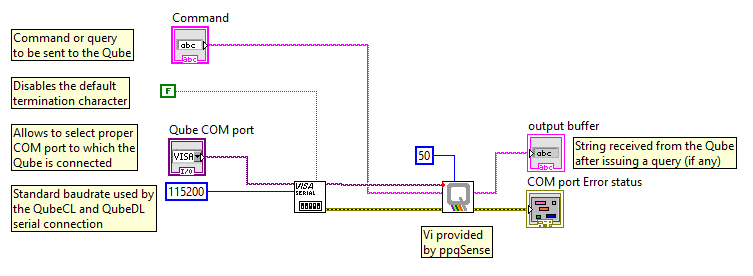
\includegraphics[width=15cm]{images/LabVIEW_VI_example.png}
    \caption{A simple LabVIEW program using the Qube\textunderscore Serial\textunderscore Interface.vi to communicate with a Qube}
    \label{LabVIEW_VI_example}
\end{figure}

\paragraph{} The Qube\textunderscore Serial\textunderscore Interface.vi needs a few inputs:
\begin{itemize}
    \item \textbf{Serial Port:} The serial port to which the Qube is connected, properly set up to work at 115200 baud without any termination character.
    \item \textbf{VISA Error:} The error for the VISA COM port made available by LabVIEW
    \item \textbf{Command:} A string containing the command with the \textbf{[identifier]:[value]} format to be sent to the Qube
    \item \textbf{Milliseconds to wait:} A constant defining how much time (in milliseconds) it is necessary to wait before accessing the Serial Buffer to read the reply received from the Qube (if any).
\end{itemize}

\paragraph{} The Qube\textunderscore Serial\textunderscore Interface.vi add the necessary terminating character in order for the command to be correctly executed by the Qube and gives back two outputs that can be used inside the program:

\begin{itemize}
    \item \textbf{Output buffer:} A string containing the reply from the Qube. It is empty for write commands or if the query gave no reply.
    \item \textbf{COM port Error status:} A VISA COM port error variable useful to check if anything went wrong during the communication with the Qube.
\end{itemize}

\begin{figure}[h]
    \centering
    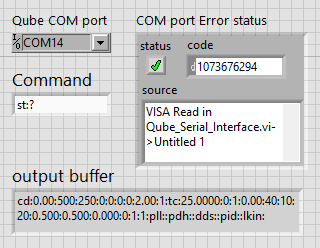
\includegraphics[width=7.5cm]{images/LabVIEW_CP_example.png}
    \caption{The panel screen of the same LabVIEW program used to send an \textbf{st:?} query to a Qube, showing the reply it sent back}
    \label{LabVIEW_CP_example}
\end{figure}


% ---------------    Python    ---------------

\subsection{Python}
\paragraph{} Python gives all the necessary tools to seamlessly connect to a Qube, sending commands and receiving replies to issued queries. As for the previous example, after a proper set up of the Serial connection, the communications is easy to implement.
\newline The example below shows a very simple function (\textit{write\textunderscore read\textunderscore from\textunderscore Qube}); it takes the command, with the \textbf{[identifier]:[value]} format, adds the necessary terminating character to it and send it to the Qube over a predefined Serial Port.
\newline The example also contains a simple script that uses the \textit{write\textunderscore read\textunderscore from\textunderscore Qube} function to perform a couple operations on the Qube.
\newline

\begin{lstlisting}[language=Python]
    import serial
    import time
    
    Qube_COM_num = "COM18"  #replace with the actual COM on your PC
    Qube_standard_Baudrate = 115200       #do not change!
    
    # initiate the serial connection
    Qube_Serial = serial.Serial(port = Qube_COM_num, baudrate = Qube_standard_Baudrate, timeout=0.6)
    
    
    
    # Basic fucntion to send commands to the Qube and receive reply to queries, if any
    def write_read_from_Qube(command):
        Qube_Serial.write(bytes(command + '\n', 'utf-8')) # adds the proper terminating character
        time.sleep(0.05)        # wait for 50 ms
        reply = Qube_Serial.readline().decode('utf8')
        return reply
    
    ########################################################################
    # Here a small demonstrative script to assess if a Qube is connected and working
    
    print("Testing the Serial Connection to the Qube")
    print("The Qube is connected to the Serial Port " + Qube_COM_num)
    print("The connection Baudrate is " + str(Qube_standard_Baudrate) + "\n")
    
    print("Issuing the command    id:?")
    Serial_number = write_read_from_Qube("id:?")
    print("The Serial Number of the Qube is: " + Serial_number)
    
    print("Checking the current status of the Qube by issuing the command   st:?\n")
    Qube_status = write_read_from_Qube("st:?")
    print("The Status of the Qube is: " + Qube_status)
    
    print("Setting the output current at 157 mA\n")
    write_read_from_Qube("iset:157")
    
    
    print("Checking if the setpoint for the output current has been received by issuing the command   st:?\n")
    Qube_status = write_read_from_Qube("st:?")
    print("The Status of the Qube is: " + Qube_status)
\end{lstlisting}

\newpage Once the proper COM port to use has been set, in this case COM18, it is possible to run the script and obtain a few information from the Qube, as shown below:

\begin{lstlisting}
    Testing the Serial Connection to the Qube
    The Qube is connected to the Serial Port COM18
    The connection Baudrate is 115200
    
    Issuing the command    id:?
    The Serial Number of the Qube is: QubeCL-185
    
    
    Checking the current status of the Qube by issuing the command   st:?
    
    The Status of the Qube is: 
        cd:810.03:900:2000:0:0:0:0:2.00:1:tc:5.0000:0:1:3.00:100:25:-10:
            0.500:0.221:0.000:1:1:1:pll::pdh::dds::pid::lkin:
    
    
    Setting the output current at 157 mA
    
    Checking if the setpoint for the output current has been received by issuing the command   st:?
    
    The Status of the Qube is:                      
        cd:157.00:900:2000:0:0:0:0:2.00:1:tc:5.0000:0:1:3.00:100:25:-10:0.500:
            0.221:0.000:1:1:1:pll::pdh::dds::pid::lkin:    
\end{lstlisting}
    \newpage
    
    \begin{versionhistory}
        \vhEntry{1.0}{2025.04.11}{LM}{First redaction.}
        \vhEntry{1.1}{2025.05.29}{LM}{Available command tables updated.}
        \vhEntry{1.2}{2025.06.06}{LM}{Available command tables updated.
                                        \newline Corrected typos in the Python example code.}
    \end{versionhistory}

\end{document}